\documentclass{article}
\usepackage{float}
\usepackage{graphicx}
\usepackage{hyperref}
\usepackage{amsmath}
\usepackage{amssymb}

\title{CCE3015 - Assignment 1 – Problem Research and Planning}
\author{Graham Pellegrini}
\date{\today}

\begin{document}

\maketitle
\section{Question 1}
The Multi-level 3D Discrete Wavelet Transform (DWT) is an effective technique in signal processing, particularly useful for data compression and denoising applications. This transform decomposes a 3D dataset into sub-bands, capturing frequency components across multiple resolutions. Each decomposition level separates the data into approximation and detail coefficients, progressively breaking down the data into low and high frequency components.

\subsection{Problem Overview}
In this problem, we will be working with the CHOAS dataset \cite{CHAOSdata2019}, which contains large 3D medical images saved as slices in DICOM (.dcm) files. Given the dataset's size and format, these slices are first pre-processed in Python to convert them into a binary (.bin) file. The preprocessing pipeline involves reading DICOM files, transforming them into NumPy arrays, and saving the arrays as binary files. This binary format will allow for efficient loading and processing in the C++ implementation of the 3D DWT.

\begin{figure}[H]
    \centering
    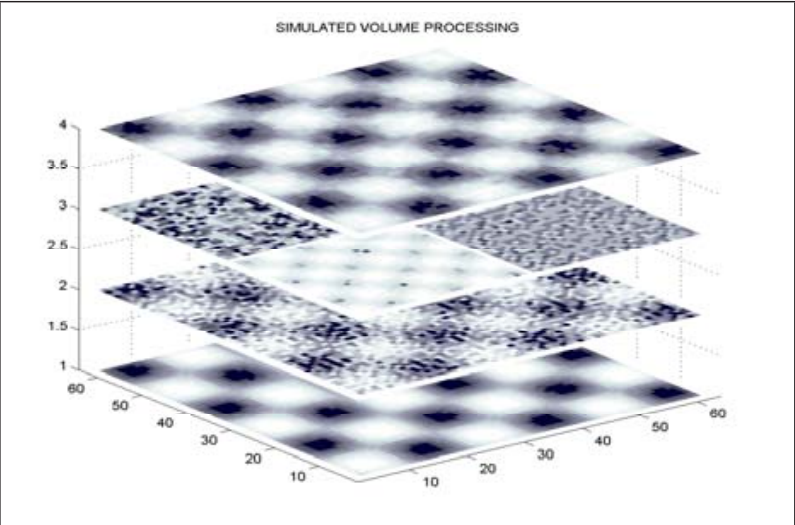
\includegraphics[width=0.9\textwidth]{assets/slices.png}
    \caption{3D Volume from 2D Slices \cite{Prochazka2011}}
    \label{fig1}
\end{figure}

In the preprocessing step, to achieve a 3D volume from 2D slices. The slices are stacked along the depth axis to form a 3D volume, as shown in Figure \ref{fig1} above. This 3D volume is saved as a numpy array in Python and then converted to a binary file for input into the C++ program. Like this the dicom slices have been converted into their respective 3D image as a volume.\\

\subsection{Algorithm Overview}
To implement the 3D DWT in C++, we will follow these key steps:\\

\textbf{Input/Output Handling} - Two utility header files will be included, one to load the binary data into a 3D volume array and another to save the processed data back into a binary file. These functions will facilitate data handling between Python and C++.\\

\textbf{Wavelet Coefficients} - Daubechies wavelet filters will be used, taking from db1 till db4. These filter coefficients will directly be sampled from pywavelets, for comparison purposes. These coefficients will be hardcoded as vectors with separation between low-pass and high-pass filters. The filters will be applied to the 3D data in the convolution step. Having the low filters and high filters separated will allow for easy implementation of the convolution step. The low emphasise the approximation coefficients and the high emphasise the detail coefficients of the signal.\\

\textbf{Discrete Wavelet Transform (DWT):} 
\begin{figure}[H]
    \centering
    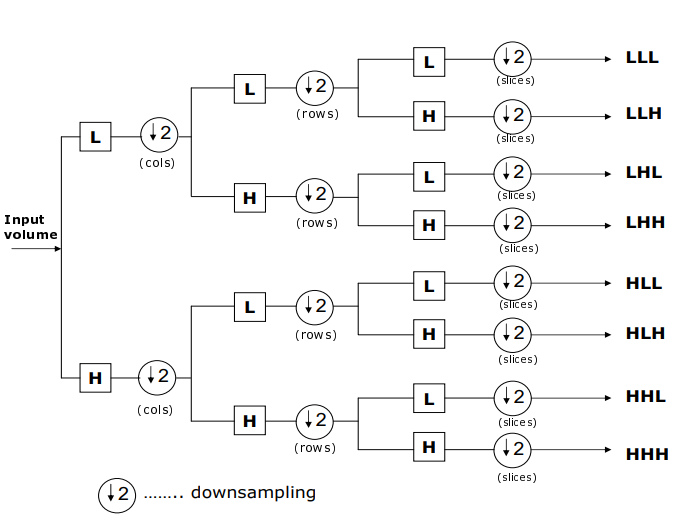
\includegraphics[width=0.8\textwidth]{assets/dwt.png}
    \caption{Discrete Wavelet Transform \cite{Prochazka2011}}
    \label{fig2}
\end{figure}

The pipeline shown in Figure \ref{fig2} shows how the 3D volume can be split into 8 subbands. However first a function to perform the 1D DWT on a signal will be defined. This function will take the signal and convolve it with the low-pass and high-pass filters. The two separated convolved outputs will then be downsampled by selecting every second value. The downsampling technique is there as a way to reduce the data size by half along each axis as well as a data redundancy reduction technique.\\

This 1D DWT function will then be called three times in the 3D DWT function, as it will be applied to each axis of the 3D volume. The 3D DWT function will take the 3D volume and apply the 1D DWT function to each axis. To keep convention the dwt is first applied to the column axis and the respective L and H subbands will be stored back to the original volume. Then the dwt is applied to the row axis and now we get the LL LH HL HH subbands. Finally the dwt is applied to the depth axis and we get the 8 subbands (LLL LLH LHL LHH HLL HLH HHL HHH). So the order 3D DWT function will include 3 nested for loops to apply the respective column-wise, row-wise and depth-wise DWT.\\

\begin{figure}[H]
    \centering
    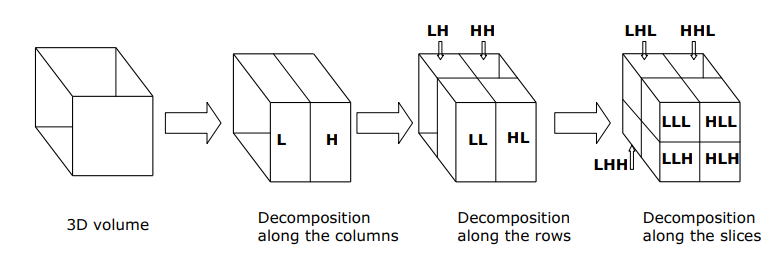
\includegraphics[width=0.8\textwidth]{assets/subbands.png}
    \caption{3D DWT Subbands \cite{Prochazka2011}}
    \label{fig3}
\end{figure}

The importance of always saving back the L and H subbands to the original volume is so we utilise memory efficiently, especially since we are working with 3d vectors of a large dataset.

\textbf{Multi-level Transform} - Our implementation aims at achieving Multi-level 3D DWT. This means we can take the approximation coefficients (LLL) from the first level and apply the 3D DWT again to get the approximation coefficients of the next level. This process can be repeated for as many levels as desired. However, it is important to note that while there is no theoretical limit to the number of levels, practical constraints are imposed by the image dimensions. In our case since the slices have dimensions of 78x256x256, a 4-level decomposition results in dimensions of 10x64x64, beyond which further decomposition would degrade image quality excessively.\\

A multi-level function will be defined that will call the 3D DWT function for the number of levels specified. If the level is not the final one then the volume dimensions will be halved along each axis, taking the approximation coefficients (LLL) and applying the 3D DWT function to them. In this process the higher level detail coefficients are discarded but they are not needed.\\
 
To be able to handle odd dimensions, either the dimension division must handle odd numbers or the volume must be padded with zeros to make the dimensions even.\\

\subsection{Evaluation and Testing}
To evaluate the implementation, we will have a post-processing step in Python. The saved output binary file will be loaded back into Python, and the 3D volume will be reconstructed from the subbands. This reconstructed coefficients will be compared to those achieved on the same volume with pywavelets. The comparison will be both visual and quantitative, using metrics like Mean Squared Error (MSE) and Euclidean Distance. Although, we will be using the same coefficients as pywavelets, there might still be some differences in implementation. Such as the convolution, downsampling techniques and padding techniques. So the graphical comparison will be the main objective and then the statistical comparison will be a bonus to see how close the implementation is to the pywavelets implementation.\\

\pagebreak

\section{Question 2}
To plan an efficient parallel implementation of the 3D Discrete Wavelet Transform (DWT) using CUDA, we analyze the operations that can be vectorized and optimized whilst handling the issue of synchronization across the architecture.

\subsection{Identifying Parallel Operations}
In the DWT process, each dimension of the 3D volume undergoes convolution with wavelet filters. This process is currently implemented sequentially, as each dimension is processed one after the other. However, this can be parallelized by using thread blocks in CUDA to process each dimension concurrently. We note that in GPU programming, the number of threads per block and blocks in the grid is a crucial parameter that must be manually tested to find the optimal values for the particular GPU setup. At the same time, we must avoid overfitting to the GPU's capabilities as this may reduce performance from one system to another or even one dataset to another.\\

So the configured threading of the individual DWT in the 3D DWT function will be one step of the parallelization from which performance can benefit. Instead of processing individual elements of the 3D volume sequentially, we can use CUDA to launch kernels that handle the 1D DWT on different parts of the volume concurrently. This allows multiple elements of the volume to be accessed and processed in parallel, significantly improving performance.\\

Since we are parallelizing the data processing, we must revise the loops present to handle the parallel execution. By configuring the number of threads per block and blocks in the grid, we can ensure that the data is processed efficiently in parallel. This will reduce the overhead associated with sequential processing, thus enhancing efficiency.\\

The I/O operations, such as loading and saving to binary files, can also be parallelized. This involves reading the 3D volume's dimensions and allocating the required memory in the GPU's global memory. CUDA kernels can then be used to read and process the data from/to the binary file in parallel. After the kernel processes the data, it is copied back to the host memory, completing the loading or saving of the volume from/to the binary file.\\

\subsection{Required Synchronization Points}
In CUDA programming, synchronization points are necessary to ensure data consistency and correct execution order. The need for synchronization arises due to data dependencies, shared memory usage, and the sequential nature of kernel launches.\\

This is why identifying synchronization points is essential to ensure data consistency and correct execution order. Preventing race conditions and ensuring the correctness of the DWT process.\\

\textbf{Within 1D DWT Kernel} - After each stage of computation within the kernel, a synchronization point is required to ensure all threads have completed their convolution and downsampling operations before proceeding. This can be achieved by synchronizing the threads with the respective function.\\

\textbf{Between 1D DWT Kernels} - After launching the 1D DWT for rows, columns, and depth slices, synchronization is required to ensure the 1D DWT on rows is completed before starting the 1D DWT on columns, and similarly for depth slices. If this is not done, then the data will be corrupted as the next DWT will be applied to the data before the previous DWT has been applied. This synchronization point will essentially have to slow down the process with a theoretical wait but is a necessary step coming from the algorithms' sequential nature.\\

\textbf{Multi-Level DWT} - Between levels in the multi-level function, synchronization is required to ensure the DWT for the current level is completed before resizing the volume and starting the next level. This is important as the data from the previous level is required to be processed in the next level. Once again this comes from the sequential nature of the algorithm and the need to process the data in a specific order.\\

Both the multi-level synchronization and the between 1D DWT kernels synchronization can be handled by synchronizing the cuda threaded devices with the respective function.\\ 

\subsection{Sequenced Plan for CUDA Implementation}
Following the above analysis, we can outline a sequenced plan for the CUDA implementation of the 3D DWT process:

\textbf{Handling I/O Operations} - The I/O operations, such as loading and saving the 3D volume data, will be handled by CUDA functions that read and write data from/to binary files. The loading in particular will handle the data to be loaded into the GPU's global memory. This sets up the data for parallel processing using CUDA and involves allocating memory on the GPU and copying the data from the host to the device.\\

\textbf{Performing 1D DWT on Rows, Columns, and Depth Slices} - The 1D DWT will be applied to the rows, columns, and depth slices of the 3D volume concurrently using CUDA kernels. Each kernel will process a row, column, or depth slice of the volume, applying the 1D DWT using wavelet filters. Synchronization within the kernel will be achieved to ensure correct execution order.\\
   
\textbf{Multi-Level DWT} - The multi-level DWT function will be implemented using CUDA, applying the 3D DWT multiple times to achieve multi-level decomposition. Handling the halving of the dimensions between levels and synchronization points to ensure data consistency and correct execution order.\\

\textbf{Selecting Block and Thread Sizes} - Once a stable implementation is achieved, the number of threads per block and blocks in the grid will be manually tested to find the optimal values for the particular GPU setup. This will involve testing different configurations to maximize GPU utilization while avoiding overfitting to the GPU's capabilities.\\

By mapping these functions to the CUDA architecture, we can leverage the parallel processing capabilities of the GPU to significantly improve the performance of the DWT process on a 3D volume. Synchronization points are carefully placed to ensure data consistency and correct execution order, preventing race conditions and ensuring the correctness of the DWT process.\\

\pagebreak

\section{Question 3}
The project is set up using a Makefile to compile the C++ code, having both a debug and release mode to compile the code. The Makefile will also have a clean function to remove the compiled files, as well as an extra check\_headers function to check if libraries other than the specified C++ STL and the Boost C++ libraries are being used.\\
\begingroup
\tiny {Use of GitHub Co-Pilot in syntax coding \cite{Copilot2024}}
\endgroup

\begin{figure}[H]
    \centering
    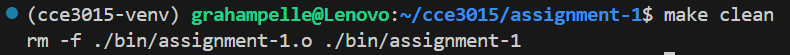
\includegraphics[width=1.2\textwidth]{assets/make_clean.png}
    \caption{make clean}
    \label{fig4}
\end{figure}

Your typical C++ file hierarchy system is being used here with src, include and bin. The "make clean" terminal command will remove the object and executable files from the bin directory.\\

\begin{figure}[H]
    \centering
    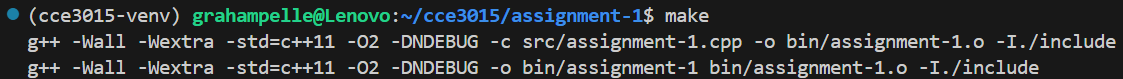
\includegraphics[width=1.2\textwidth]{assets/make.png}
    \caption{make}
    \label{fig5}
\end{figure}

\begin{figure}[H]
    \centering
    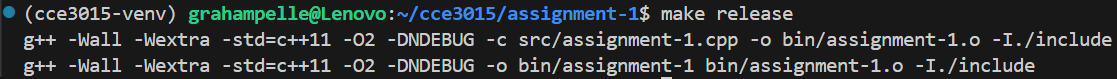
\includegraphics[width=1.2\textwidth]{assets/make_release.png}
    \caption{make release}
    \label{fig6}
\end{figure}

Figure \ref{fig5} and Figure \ref{fig6} show the same make operation since the release mode is the default mode. These makes do not provide debugging information and enable optimizations with the "-O2" flag to the compiler. It also disables assertions with the "-DNDEBUG" flag, so the code will run faster without any debugging information.\\

\begin{figure}[H]
    \centering
    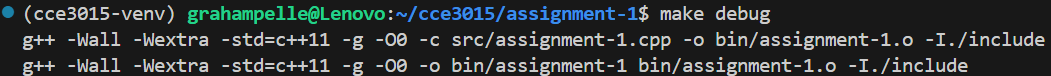
\includegraphics[width=1.2\textwidth]{assets/make_debug.png}
    \caption{make debug}
    \label{fig7}
\end{figure}

Figure \ref{fig7} shows the make operation for the debug mode. This mode provides debugging information "-g" and disables optimizations with the "-O0" flag to the compiler.\\

\begin{figure}[H]
    \centering
    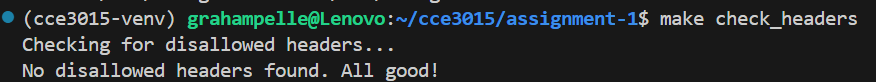
\includegraphics[width=1.2\textwidth]{assets/make_check_headers.png}
    \caption{make check\_headers}
    \label{fig8}
\end{figure}

The "make check\_headers" is an extra function that checks if any libraries other than the specified C++ STL and the Boost C++ libraries are being used. This is to ensure that the code will run on the university's system and not include any external libraries that are not allowed for the scope of the assignment.\\

\begin{itemize}
    \item -- All compiler warnings have been resolved --
    \item -- The code accepts an input and output binary file --
    \item -- The code runs for any number of levels of decomposition --
    \item -- The code is limited to db 1 to db 4 wavelet filters, throwing an assert when another filter number is used --
    \item -- Timing information is printed to the console for the DWT process and the total time including I/O operations --
    \item -- The code has been tested on the university's system and runs without any errors --
\end{itemize}

\pagebreak

\section{Question 4}

Note all timings are achieved using home system CPU. The GPU where naturally different and found to be slower. However, the GPU timings will later be useful to compare to when the CUDA implementation is complete and it is expected to be faster than the current CPU timings.\\

\subsection{1 Level db1}
\begin{itemize}
    \item -- DWT Time: 0.000000s --
    \item -- Total Time: 0.000000s --
\end{itemize}

\begin{figure}[H]
    \centering
    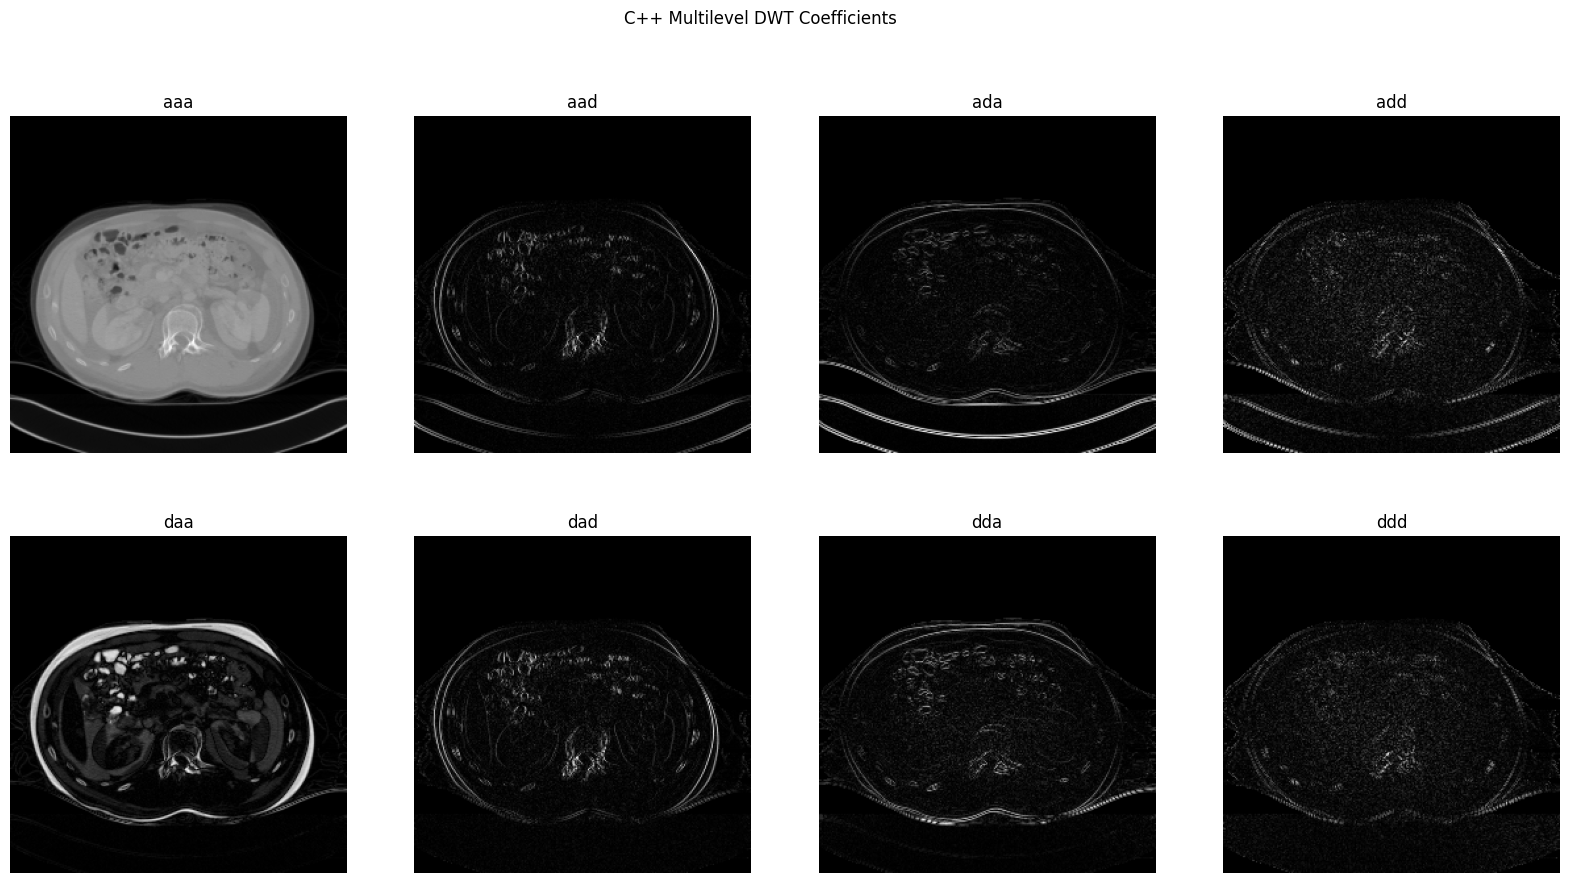
\includegraphics[width=0.8\textwidth]{assets/cpp-1-db1.png}
    \caption{C++ 1 Level db1}
    \label{fig9}
\end{figure}

\begin{figure}[H]
    \centering
    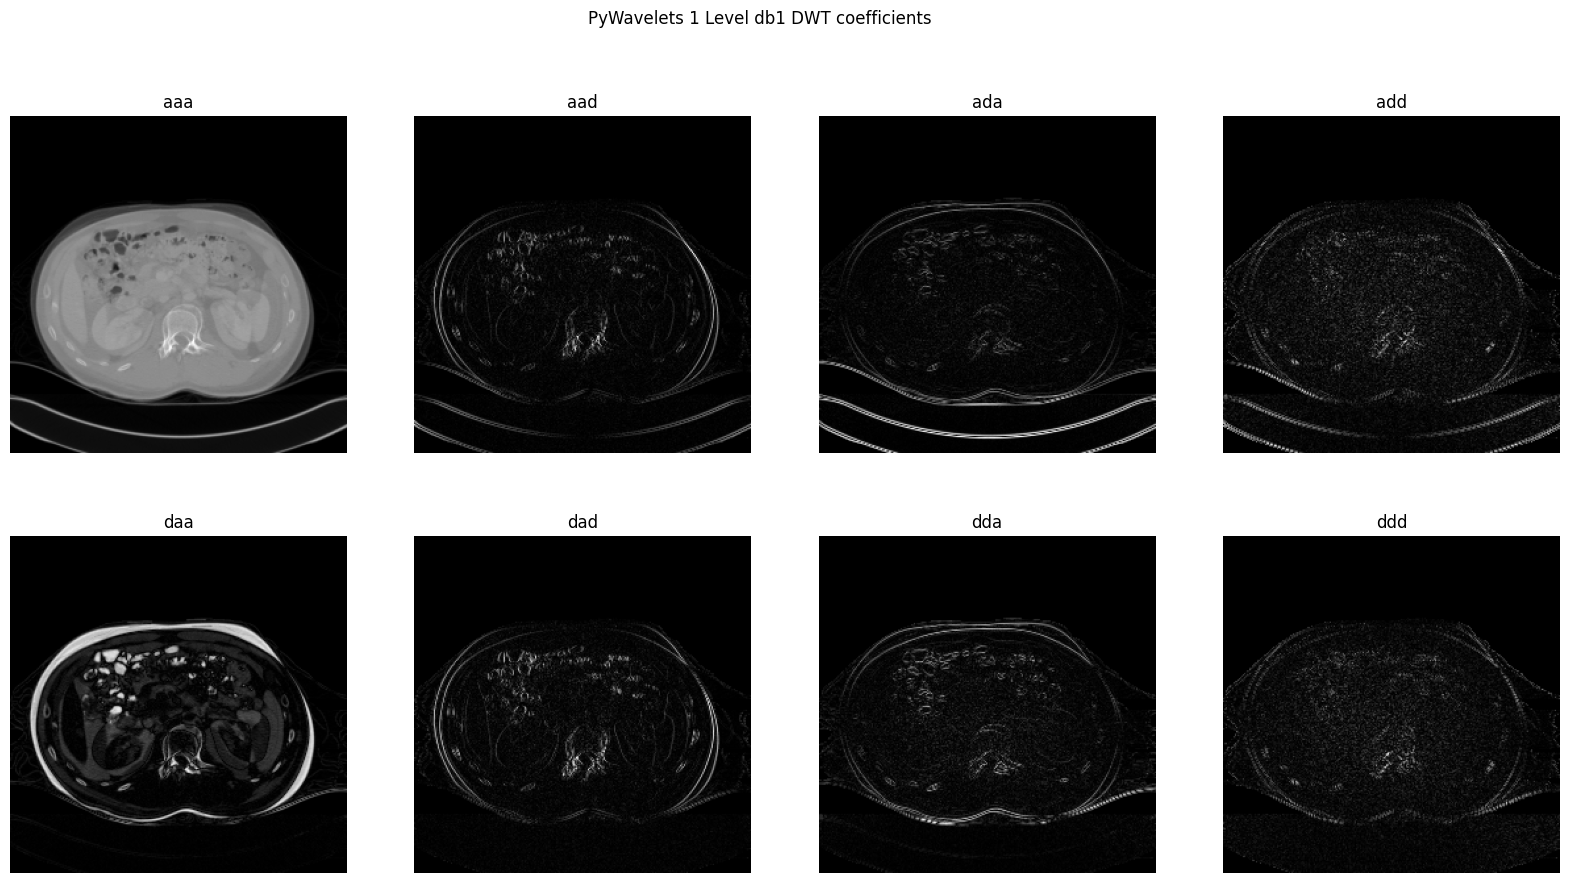
\includegraphics[width=0.8\textwidth]{assets/py-1-db1.png}
    \caption{Python 1 Level db1}
    \label{fig10}
\end{figure}

\begin{itemize}
    \item Subband aaa - MSE: 5.184754738713458e-15, Euclidean Distance: 0.00011511619231896475
    \item Subband aad - MSE: 1.237035213846882e-12, Euclidean Distance: 0.0017780977068468928
    \item Subband ada - MSE: 5.124077702943486e-13, Euclidean Distance: 0.0011443720431998372
    \item Subband add - MSE: 7.0118897667337254e-12, Euclidean Distance: 0.004233064129948616
    \item Subband daa - MSE: 3.29426664712109e-14, Euclidean Distance: 0.00029016935150139034
    \item Subband dad - MSE: 9.42445448938456e-14, Euclidean Distance: 0.000490792328491807
    \item Subband dda - MSE: 9.70302289036995e-13, Euclidean Distance: 0.0015747473808005452
    \item Subband ddd - MSE: 2.938679302070396e-13, Euclidean Distance: 0.0008666514186188579
\end{itemize}

\subsection{1 Level db2}
\begin{itemize}
    \item -- DWT Time: 0.000000s --
    \item -- Total Time: 0.000000s --
\end{itemize}


\begin{figure}[H]
    \centering
    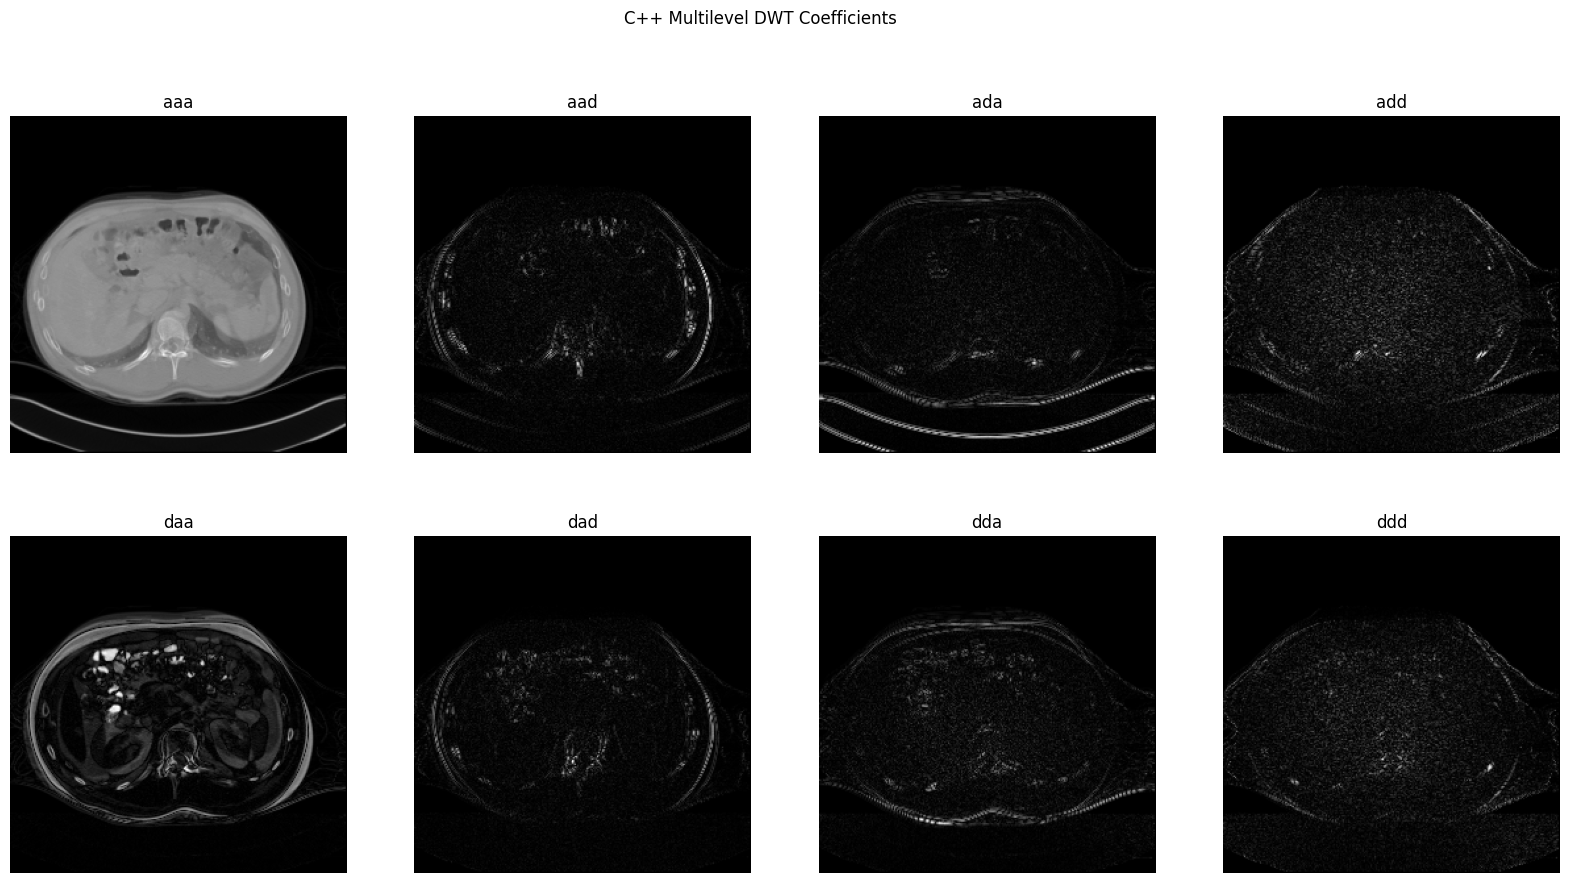
\includegraphics[width=0.8\textwidth]{assets/cpp-1-db2.png}
    \caption{C++ 1 Level db2}
    \label{fig11}
\end{figure}

\begin{figure}[H]
    \centering
    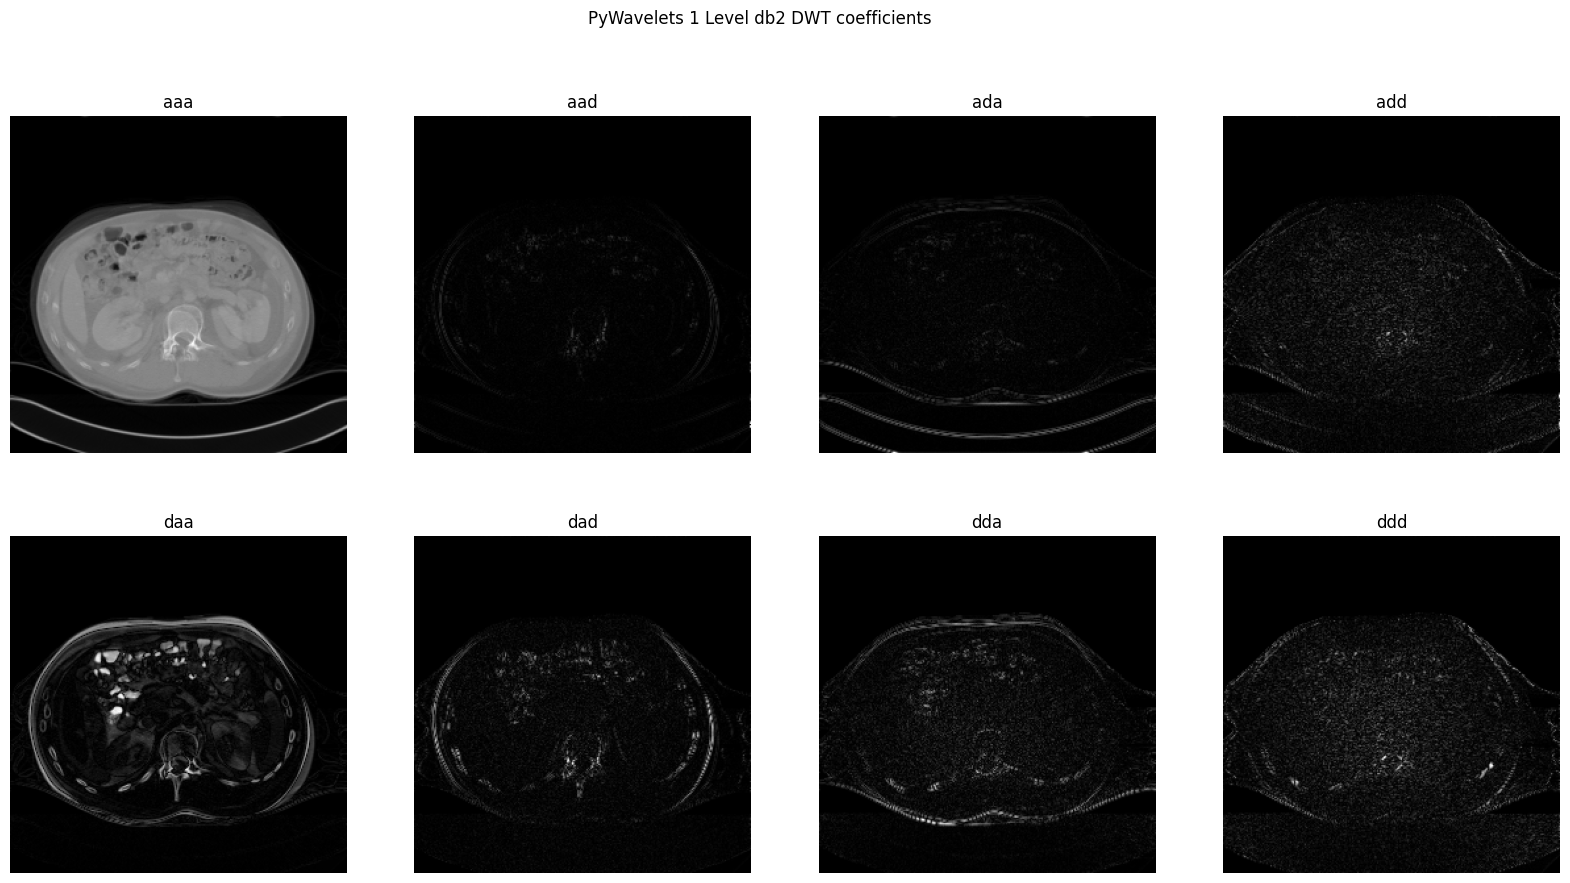
\includegraphics[width=0.8\textwidth]{assets/py-1-db2.png}
    \caption{Python 1 Level db2}
    \label{fig12}
\end{figure}

\begin{itemize}
    \item Subband aaa - MSE: 0.34114518761634827, Euclidean Distance: 933.7196655273438
    \item Subband aad - MSE: 1.3752477169036865, Euclidean Distance: 1874.7982177734375
    \item Subband ada - MSE: 0.8219887018203735, Euclidean Distance: 1449.444580078125
    \item Subband add - MSE: 1.2700697183609009, Euclidean Distance: 1801.6768798828125
    \item Subband daa - MSE: 0.4385218620300293, Euclidean Distance: 1058.6290283203125
    \item Subband dad - MSE: 0.8035810589790344, Euclidean Distance: 1433.107421875
    \item Subband dda - MSE: 0.8032531142234802, Euclidean Distance: 1432.7926025390625
    \item Subband ddd - MSE: 0.5720685720443726, Euclidean Distance: 1209.139404296875
\end{itemize}

\subsection{2 Levels db3}
\begin{itemize}
    \item -- DWT Time: 0.000000s --
    \item -- Total Time: 0.000000s --
\end{itemize}

\begin{figure}[H]
    \centering
    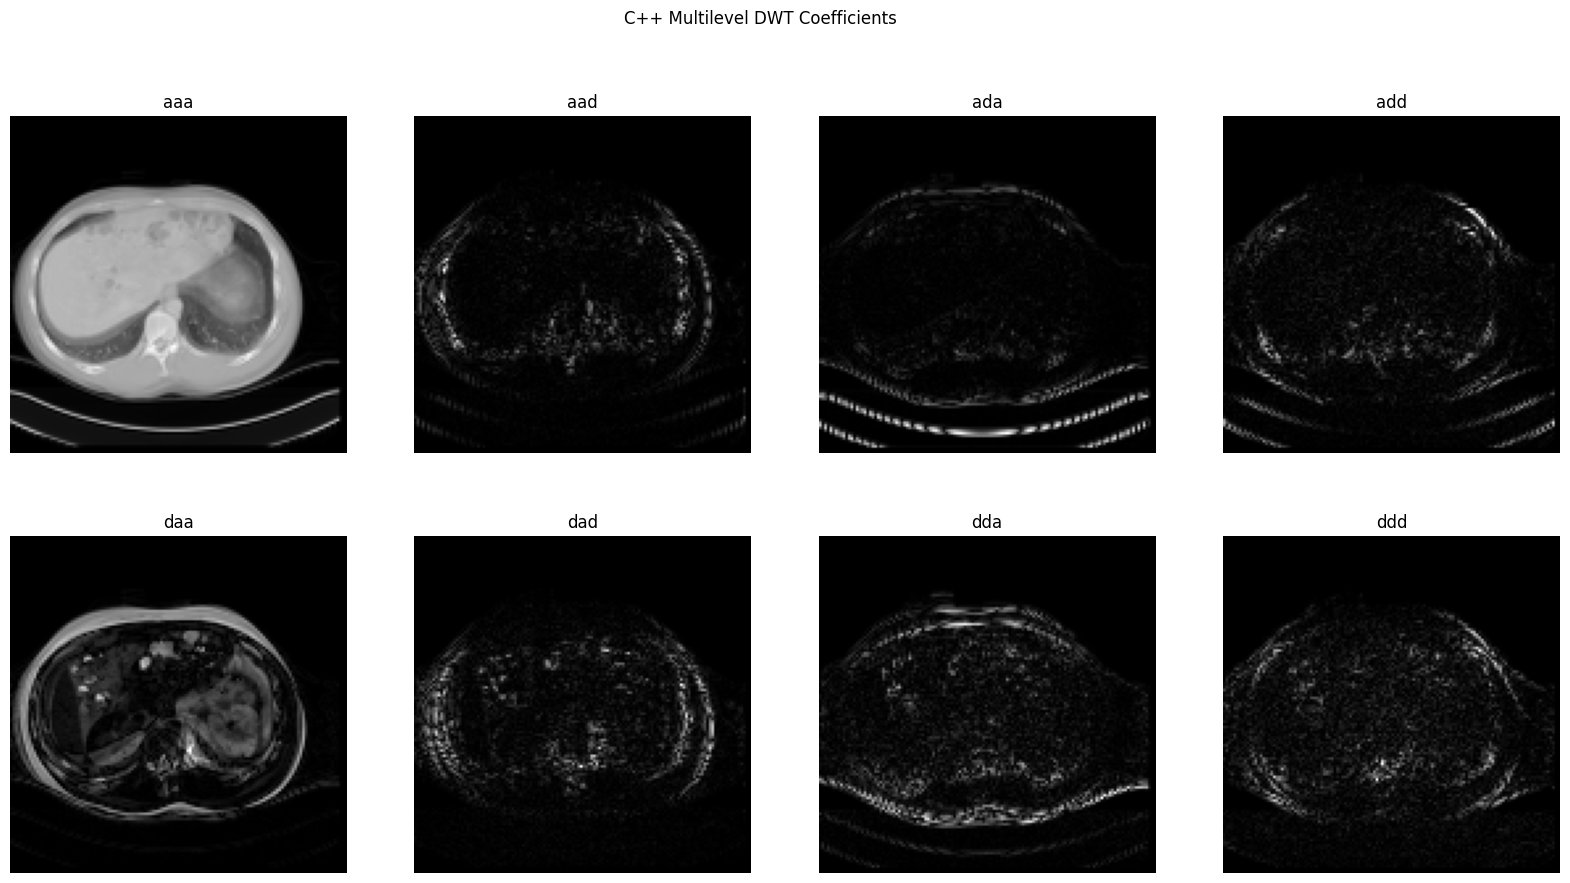
\includegraphics[width=0.8\textwidth]{assets/cpp-2-db3.png}
    \caption{C++ 2 Levels db3}
    \label{fig13}
\end{figure}

\begin{figure}[H]
    \centering
    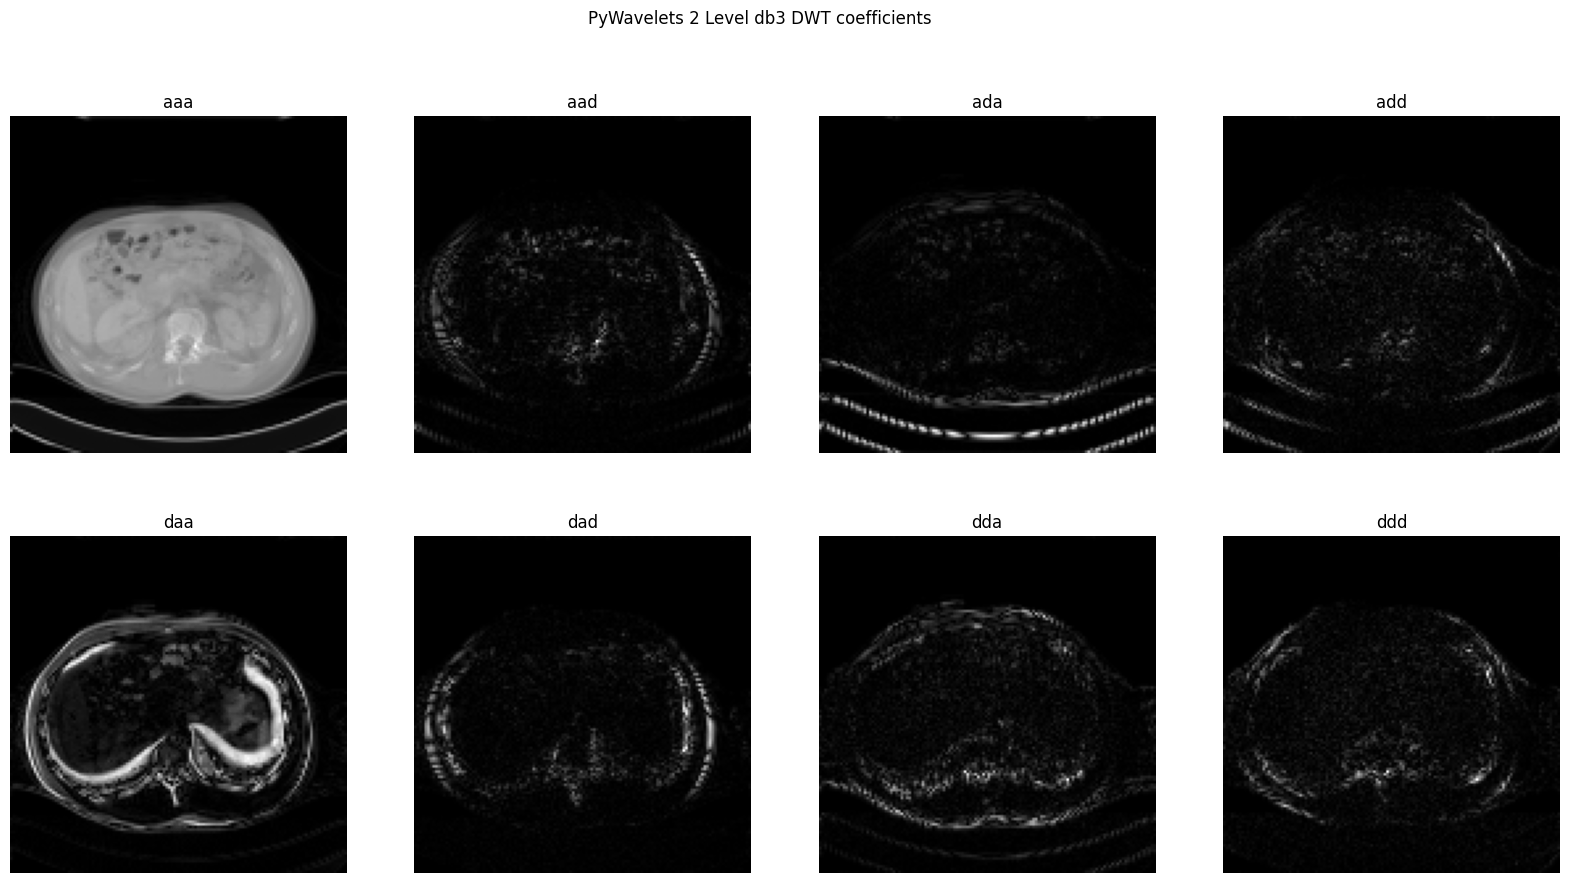
\includegraphics[width=0.8\textwidth]{assets/py-2-db3.png}
    \caption{Python 2 Levels db3}
    \label{fig14}
\end{figure}

\begin{itemize}
    \item Subband aaa - MSE: 0.5933269262313843, Euclidean Distance: 440.9319763183594
    \item Subband aad - MSE: 1.3555747270584106, Euclidean Distance: 666.4804077148438
    \item Subband ada - MSE: 1.3116660118103027, Euclidean Distance: 655.5968627929688
    \item Subband add - MSE: 1.2220373153686523, Euclidean Distance: 632.8031616210938
    \item Subband daa - MSE: 1.3143343925476074, Euclidean Distance: 656.2611083984375
    \item Subband dad - MSE: 1.300540804862976, Euclidean Distance: 652.8126220703125
    \item Subband dda - MSE: 1.2866054773330688, Euclidean Distance: 649.3057861328125
    \item Subband ddd - MSE: 1.2334144115447998, Euclidean Distance: 635.7376708984375
\end{itemize}

\subsection{3 Levels db2}
\begin{itemize}
    \item -- DWT Time: 0.000000s --
    \item -- Total Time: 0.000000s --
\end{itemize}


\begin{figure}[H]
    \centering
    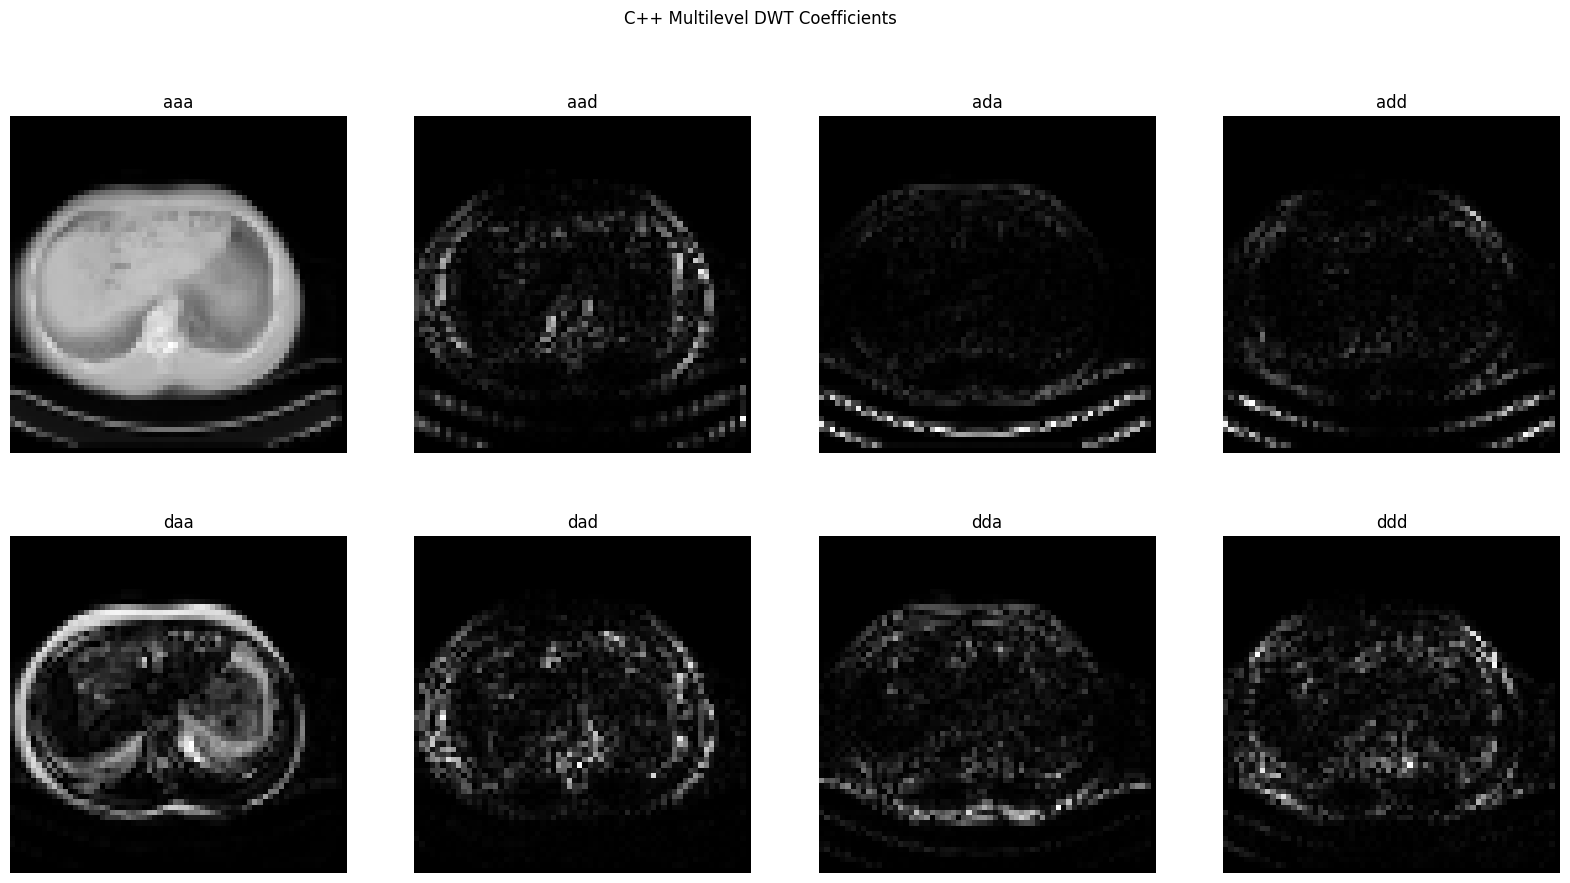
\includegraphics[width=0.8\textwidth]{assets/cpp-3-db2.png}
    \caption{C++ 3 Levels db2}
    \label{fig15}
\end{figure}

\begin{figure}[H]
    \centering
    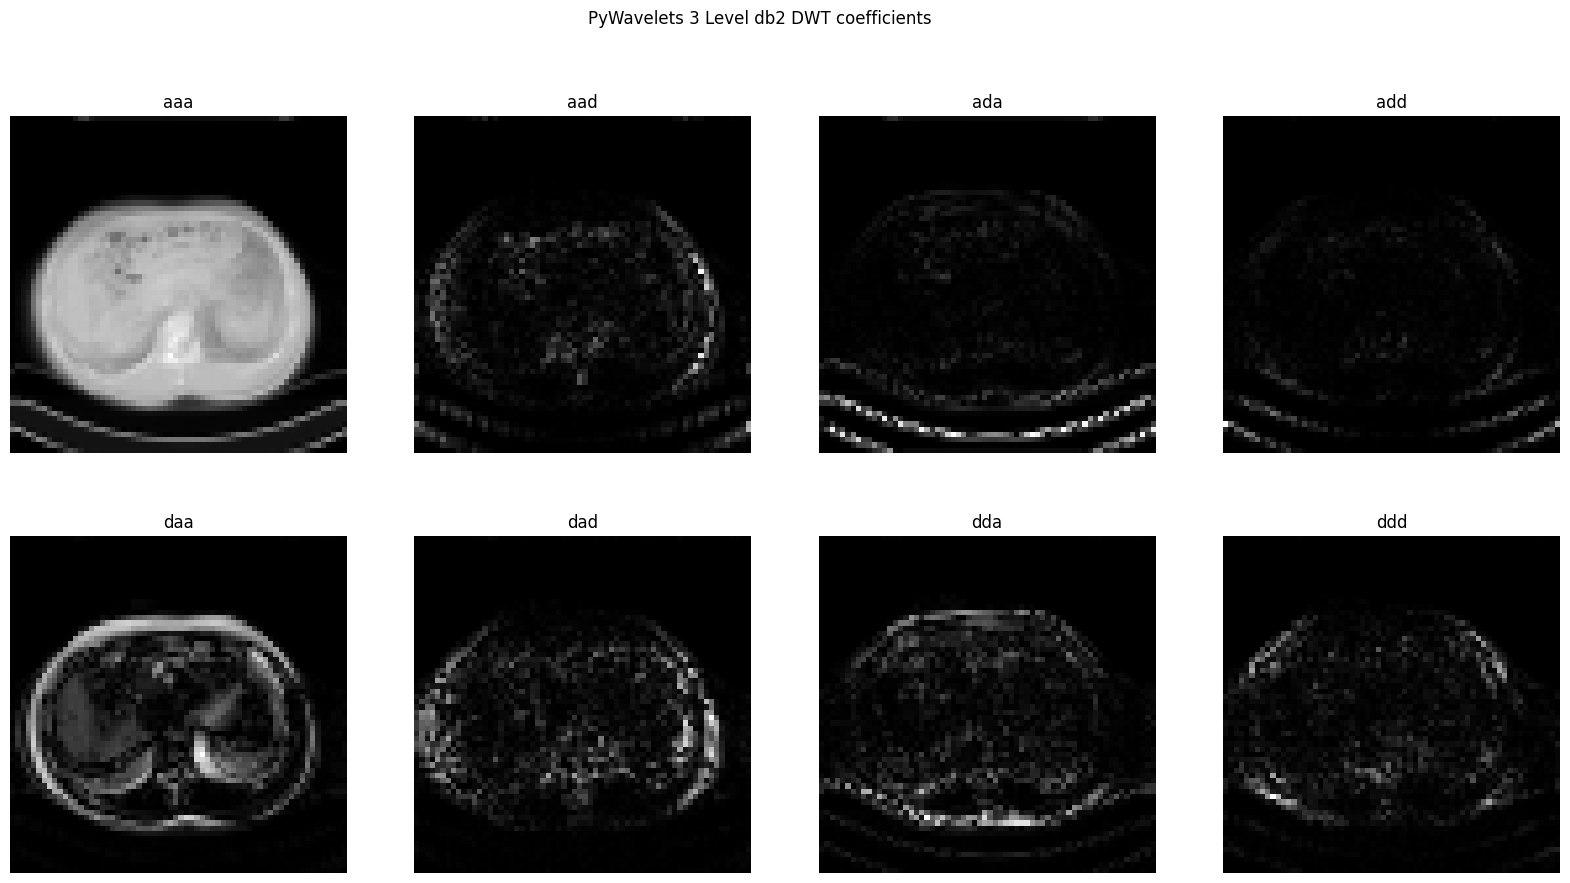
\includegraphics[width=0.8\textwidth]{assets/py-3-db2.png}
    \caption{Python 3 Levels db2}
    \label{fig16}
\end{figure}

\begin{itemize}
    \item Subband aaa - MSE: 0.6106096506118774, Euclidean Distance: 158.14723205566406
    \item Subband aad - MSE: 1.35321044921875, Euclidean Distance: 235.4304962158203
    \item Subband ada - MSE: 1.3130872249603271, Euclidean Distance: 231.913818359375
    \item Subband add - MSE: 1.164674162864685, Euclidean Distance: 218.41477966308594
    \item Subband daa - MSE: 1.380114197731018, Euclidean Distance: 237.7592315673828
    \item Subband dad - MSE: 1.256959080696106, Euclidean Distance: 226.9029998779297
    \item Subband dda - MSE: 1.3253566026687622, Euclidean Distance: 232.99488830566406
    \item Subband ddd - MSE: 1.2182940244674683, Euclidean Distance: 223.3861846923828
\end{itemize}

\pagebreak

\bibliographystyle{ieeetr}
\bibliography{references.bib}
\end{document}